\documentclass{gescons}

\genre {Entrevista}
\author{Cristina Bassanesi}
\title{O Calidoscópio da Evolução Consciencial: Abordagem Interparadigmática da Evoluciologia}


\begin{document}
    \makeentrevistatitle
    \coverart{back/Cristina_Bassanesi}

    \begin{multicols}{2}

\subsubsection{1. Qual foi a motivação para a escrita da obra? Por que a definição deste tema para publicação de um livro?}

Esta obra teve como motivação escrever sobre a \textit{Mutabilidade Consciencial Não Linear,} tema pertinente à \textit{Especialidade Evoluciologia,} empregando abordagem científica, multidisciplinar e interparadigmática.

A definição pelo tema somente foi estabelecida em definitivo após o movimento pessoal de começar a escrever. O roteiro previamente delineado mudou logo no início, quando ampliei a cosmovisão sobre o que poderia ser o tema central do livro e passei a aplicar \textit{o princípio de os fatos e parafatos orientarem a pesquisa.}

\subsubsection{2. Quais foram as principais percepções, intra e extrafísicas, durante a pesquisa e a escrita da obra? E posterior ao lançamento?}

Atitude pessoal determinante para manter a rotina de escrita foi o autoposicionamento de priorizar 1 turno fixo do dia (manhã) para à escrita, em detrimento dos inúmeros apelos para envolvimento em outras atividades. Nesse ponto, a sobreveniência do desassédio mentalsomático e a parapercepção do amparo de função, atuando tanto com inspirações quanto no auxílio à resolução de entraves dos mais variados tipos tornou-se evidente.

As repercussões favoráveis do livro publicado trouxeram grande alegria, porém, com maior intensidade, asseveraram o autocompromisso intermissivo com a tares autoral. 

\begin{pullquote}
``As repercussões favoráveis do livro publicado trouxeram grande alegria, porém, com maior intensidade, asseveraram o autocompromisso intermissivo com a tares autoral.''
\end{pullquote}

\subsubsection{3. Qual o maior aprendizado com a escrita desta obra?}

Sem dúvida, a conclusão da obra deixou saldo de aprendizados, dentre os quais destaco o valor do exercício da persistência e paciência na sustentação gesconográfica. Aprendizado adicional foi o de eliminar o apego a ideias, frases e até vocábulos, que a princípio podem soar muito boas. Contudo, por vezes, atravancam durante horas ou dias a fluidez da escrita. A sugestão é guardá-las em algum arquivo próprio, para utilização em outra oportunidade. 

\begin{pullquote}
``Sem dúvida, a conclusão da obra deixou saldo de aprendizados, dentre os quais destaco o valor do exercício da persistência e paciência na sustentação gesconográfica.''
\end{pullquote}

\subsubsection{4. O que poderia dizer como incentivo para que mais pesquisadores invistam na publicação de obras conscienciológicas?}

Deixo o incentivo, aos potenciais escritores, a investirem na escrita de obras conscienciológicas, expondo as autossingularidades ou especialidades pessoais, as quais podem trazer novos vieses de compreensão sobre a evolução consciencial e novas senhas aos neointermissivistas. 

    %\noindent\includegraphics[width=11cm, height=12cm]{example-image} 

\begin{center}
    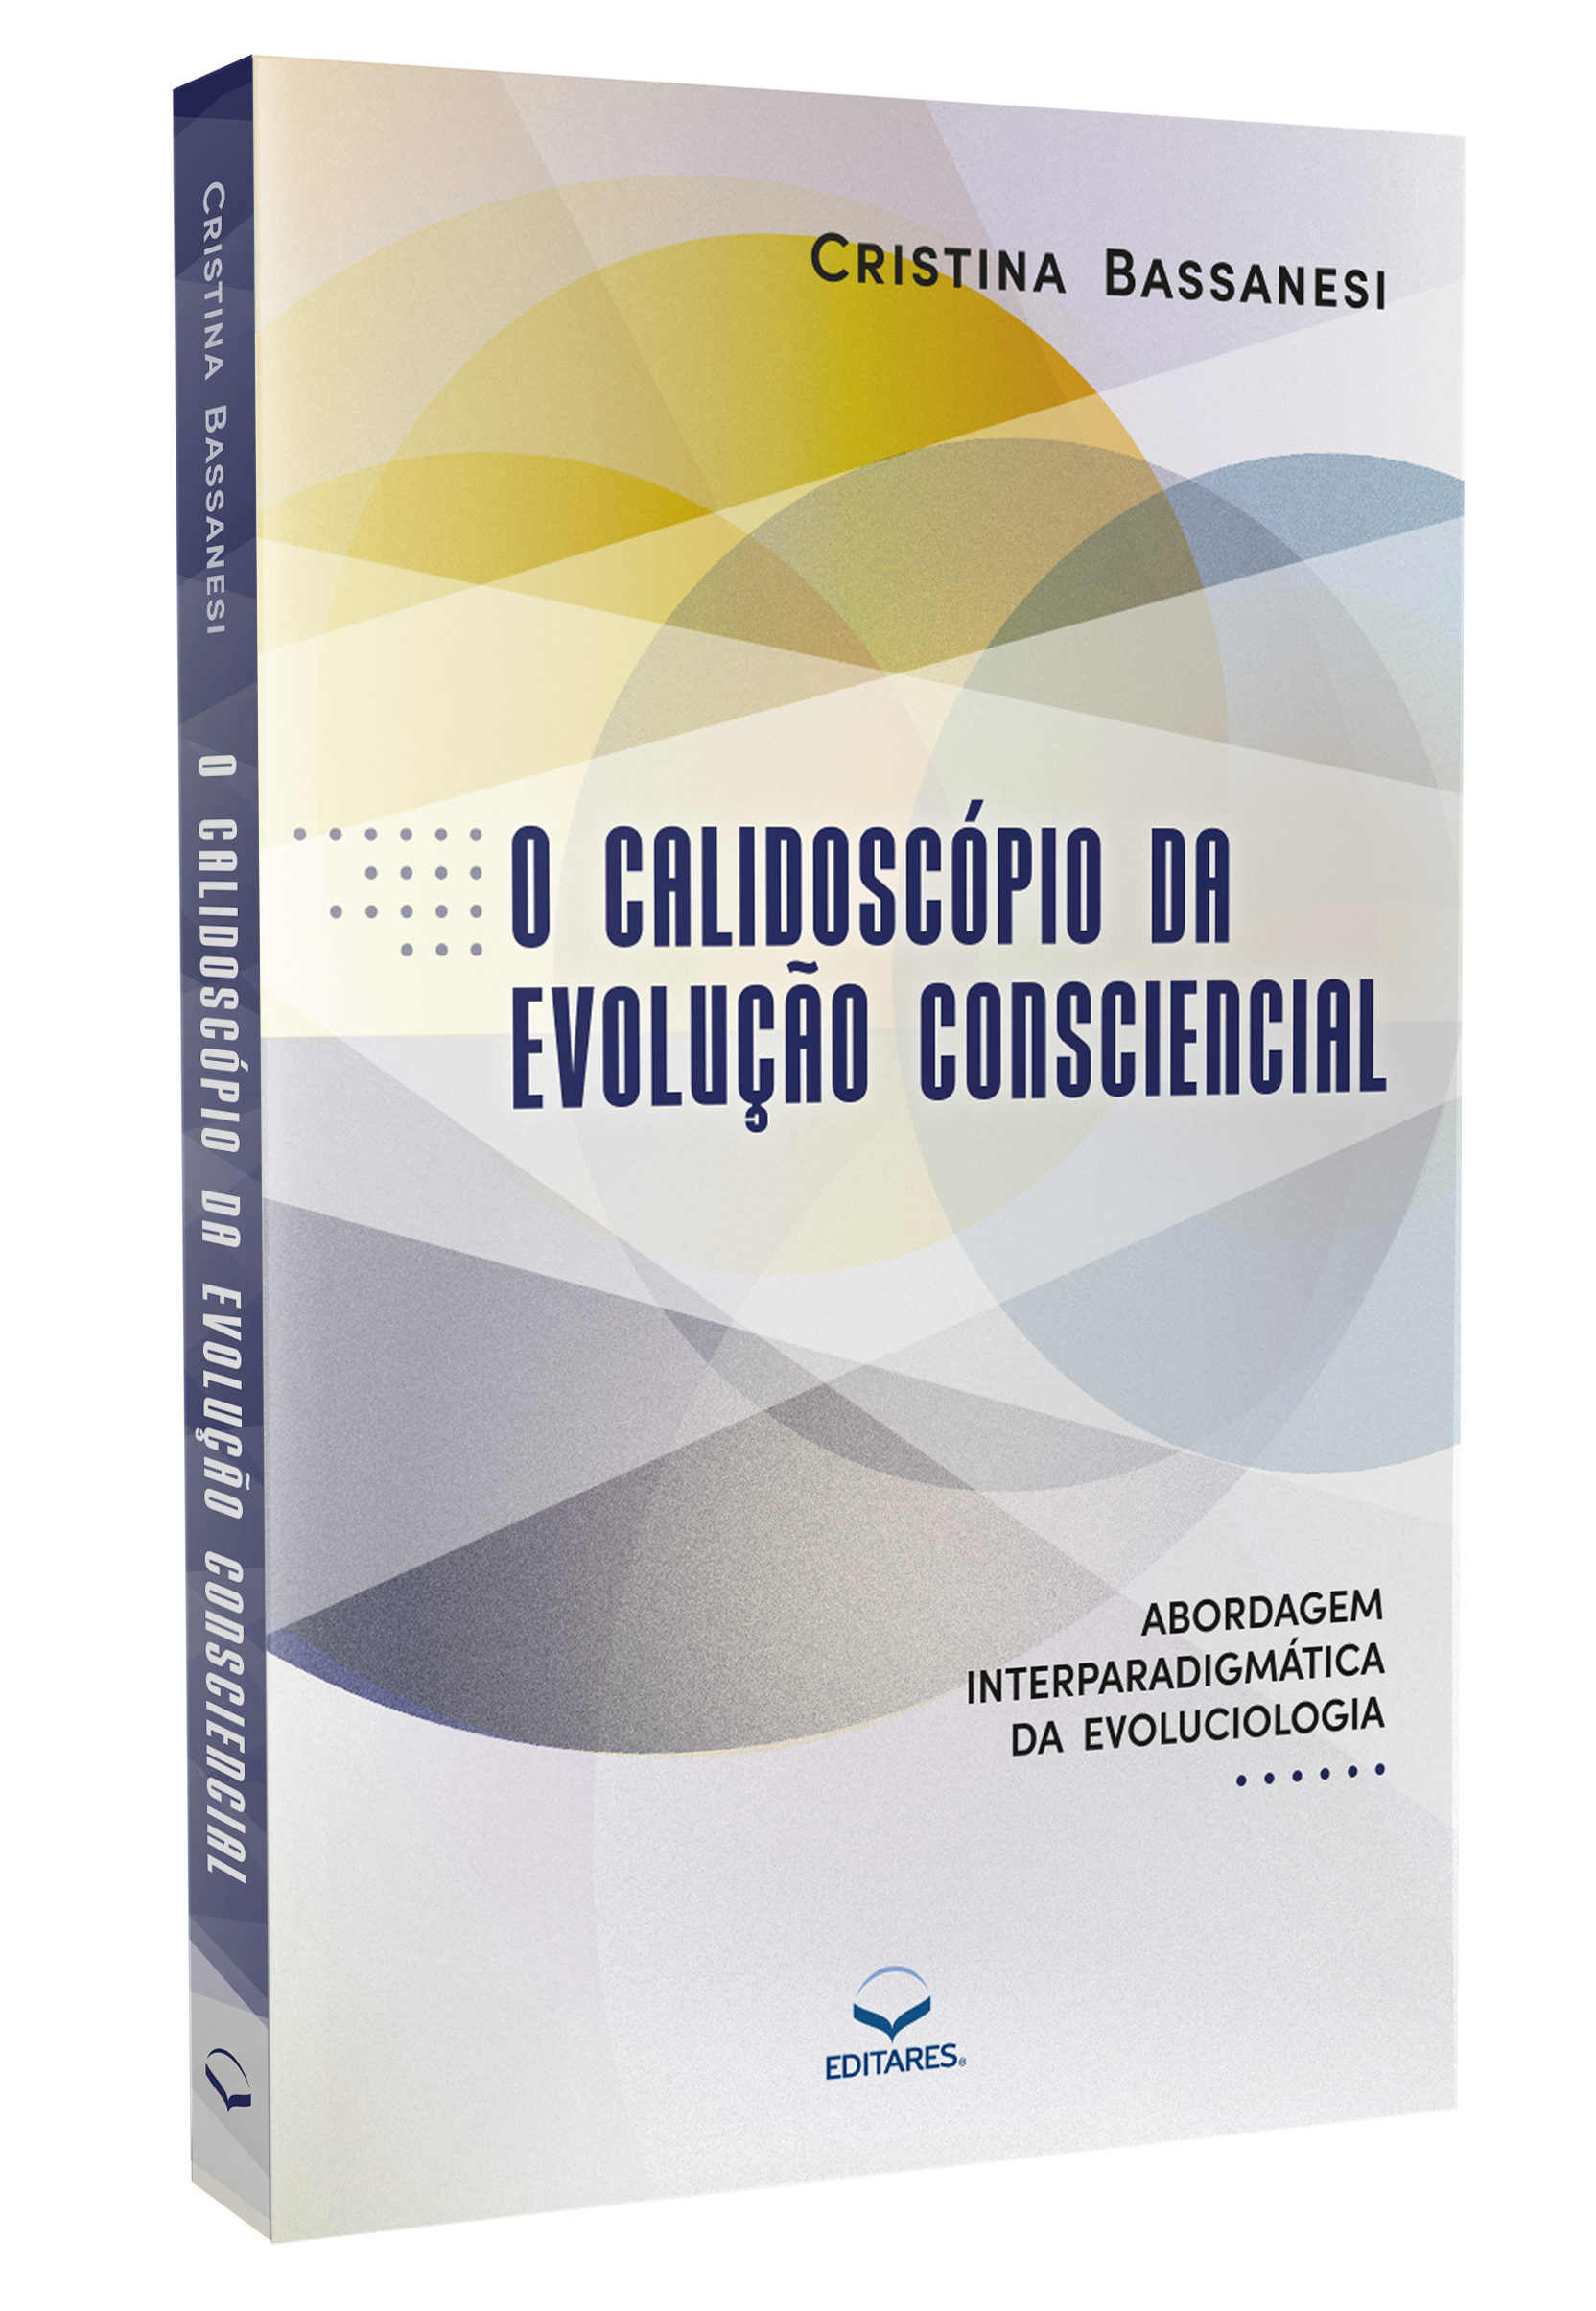
\includegraphics[width=8cm]{articles/entrevista/mockups/Cristina-Bassanesi.png}
    %\noindent\includegraphics[width=8cm, height=10cm]{example-image}
\end{center}
    
    \end{multicols}
\end{document}
